\documentclass[11pt]{article}
\usepackage[margin=1in]{geometry}
\usepackage{amsmath, amssymb, amsthm}
\usepackage{graphicx}
\usepackage{booktabs}
\usepackage{longtable}
\usepackage{microtype}
\usepackage{xspace}
\usepackage{xcolor}
\usepackage{hyperref}
\usepackage[numbers, sort&compress]{natbib}

\newtheorem{theorem}{Theorem}
\newtheorem{corollary}{Corollary}
\newtheorem{definition}{Definition}

\newcommand{\excalibr}{ExCALIBR\xspace}
\newcommand{\postp}{P(Y{=}1\mid E{=}e)}
\newcommand{\lrp}{\mathrm{LR}^{+}}

\title{\textbf{Prior-adaptive evidence thresholds for clinical variant classification:\\
       limitations of the Tavtigian framework and a piecewise Bayesian solution}}
\author{}
\date{}

\begin{document}
\maketitle

\begin{abstract}
\noindent
Evidence-based variant classification under the ACMG/AMP guidelines requires
mapping continuous likelihood-ratio scores to discrete evidence strengths using
thresholds that satisfy specified posterior probability targets.
The Tavtigian et al.\ framework provides such thresholds through a single
constant $C^*$ calibrated to a canonical prior of $p = 0.10$, but the
mapping is exact only at that prior and degrades systematically at all others.
We characterise the failure modes of this approach in detail:
pathogenic thresholds drift from their targets at priors above ${\sim}0.20$,
while benign thresholds are severely miscalibrated across the entire
biologically relevant range---at $p = 0.01$, the LB boundary posterior is
$0.003$ instead of $0.10$, causing benign evidence to be withheld from the
vast majority of variants that should receive it.
We prove that no additive scoring system with prior-independent thresholds can
simultaneously produce exact posteriors at all classification boundaries for all
priors, and we show that a piecewise-linear Bayesian solution achieves exact
boundary posteriors at every prior while preserving the ACMG/AMP point system.
We demonstrate that the threshold difference is practically large: at $p=0.01$,
the piecewise LB threshold (LR$^+{<}11$) is 42$\times$ more permissive than
the Tavtigian threshold (LR$^+{<}0.26$), directly reducing false-negative
benign evidence assignments in assay calibration pipelines.
\end{abstract}

% ------------------------------------------------------------------
\section*{Introduction}
% ------------------------------------------------------------------

The ACMG/AMP guidelines~\cite{richards2015standards} classify genetic variants
into five categories according to their posterior probability of pathogenicity:
pathogenic ($\geq$99\%), likely pathogenic (LP; $\geq$90\%), uncertain
significance (10--90\%), likely benign (LB; $\leq$10\%), and benign
($\leq$1\%).
Classification combines independent lines of evidence, each characterised by
a direction (pathogenic or benign) and strength (supporting, moderate, strong,
or very strong), according to fixed combination rules~\cite{richards2015standards}.
Tavtigian et al.~\cite{tavtigian2018modeling, Tavtigian2020} formalised this as
a Bayesian point system in which each evidence strength carries an integer
point value ($\pm1$, $\pm2$, $\pm4$, $\pm8$) proportional to $\log(\lrp)$ (the natural
logarithm of the likelihood ratio), so that the combined $\lrp$ for total points $T$ is
$\lrp(T) = C^{T/8}$ for a single constant $C = O_{\mathrm{PVSt}}$.

Evidence calibration pipelines---including our own
\excalibr~\cite{igvf_pp}---convert continuous assay scores to evidence points by
comparing the variant's score-specific $\lrp$ to the thresholds
$C^{k/8}$ for each evidence strength $k \in \{1,2,4,8\}$.
Supporting evidence requires $\lrp(s) \geq C^{1/8}$; moderate requires
$\lrp(s) \geq C^{1/4}$; and so on~\cite{pejaver2022calibration}.
These thresholds are correct only if the posterior probability at each
boundary satisfies the ACMG target---that is, only if the correct $C$ is used
for the gene-specific prior.
However, $C^*$ in the Tavtigian framework is a single integer determined by
grid search at the canonical prior $p = 0.10$, and applying it at other priors
yields thresholds that map assay scores to incorrect posterior probabilities.

Harrison et al.~\cite{Harrison2019} observed that variants classified as LP
in ClinVar often carry posterior probabilities well below the nominal 90\%,
and that reclassification data reveal systematic inconsistency in posterior
calibration across genes.
A key source of this inconsistency is the prior-dependence of the correct
classification threshold: a variant whose $\lrp$ just reaches the LP threshold
at $p = 0.10$ would yield a posterior of only 0.45 at $p = 0.01$---squarely
in the VUS range---while the same threshold yields 0.96 at $p = 0.25$.
Functional assay calibration pipelines that apply Tavtigian thresholds without
prior-adaptation therefore produce evidence assignments whose implied posteriors
depend on the gene-specific prior in an uncontrolled way.
This is not a limitation of the underlying assay or calibration model, but of
the threshold mapping from $\lrp$ to evidence strength.

Here, we characterise the calibration errors introduced by prior-fixed Tavtigian
thresholds, prove that this limitation is unavoidable for any additive system
with prior-independent thresholds, and describe a piecewise-linear Bayesian
solution that achieves exact boundary posteriors at every prior.
We provide quantitative comparisons of evidence threshold accuracy across the
biologically relevant prior range and discuss the implications for assay
calibration pipelines such as \excalibr~\cite{igvf_pp},
OddsPath~\cite{brnich2020recommendations}, and PP3/BP4
calibration~\cite{pejaver2022calibration}.

% ------------------------------------------------------------------
\section*{The Tavtigian Framework and Its Prior-Dependent Failures}
% ------------------------------------------------------------------

\subsection*{Construction and calibration at the canonical prior}

Given a prior $p$ and a combined $\lrp = C^{T/8}$, the posterior probability of
pathogenicity is
\begin{equation}
  \postp =
  \frac{C^{T/8}\, p}{\bigl(C^{T/8} - 1\bigr)p + 1}.
  \label{eq:bayes}
\end{equation}
The constant $C$ (the ``OddsPath'' $O_{\mathrm{PVSt}}$) is determined from the
2020 derivation~\cite{Tavtigian2020}: five of the six LP combination rules
each require odds equivalent to six pieces of supporting evidence, fixing
$O_{\mathrm{PSu}}^6 = 81$, hence
$C^* = O_{\mathrm{PSu}}^8 = 81^{4/3} \approx 350$ at $p = 0.10$.
To resolve two originally inconsistent ACMG rules, we follow the modification of
Tavtigian et al.~\cite{tavtigian2018modeling}: the combination 2S is moved to the
LP classification (8 points, Post\_P $\approx$ 0.975) and VS+M is moved to the
P classification (10 points, Post\_P $\approx$ 0.994); all remaining rules are internally
consistent at $p = 0.10$ with $C^* = 350$.

\subsection*{Threshold accuracy degrades away from $p = 0.10$}

\begin{table}[t]
\centering
\caption{Tavtigian boundary posteriors vs.\ piecewise targets at five
         representative priors.
         Piecewise values are exact at each target by construction.
         $C^*$ is from the integer grid search.}
\label{tab:boundary}
\begin{tabular}{rr @{\hspace{1em}} rr @{\hspace{1em}} rr @{\hspace{1em}} rr @{\hspace{1em}} rr}
\toprule
$p$ & $C^*$
  & \multicolumn{2}{c}{LP (6 pts, tgt 0.90)}
  & \multicolumn{2}{c}{P (10 pts, tgt 0.99)}
  & \multicolumn{2}{c}{LB ($-$1 pts, tgt 0.10)}
  & \multicolumn{2}{c}{B ($-$7 pts, tgt 0.01)} \\
& & Tav & PW & Tav & PW & Tav & PW & Tav & PW \\
\midrule
0.01 & 8511  & \textbf{.900} & .900 & .999 & \textbf{.990} & .003 & \textbf{.100} & .000 & \textbf{.010} \\
0.05 &  950  & \textbf{.900} & .900 & .996 & \textbf{.990} & .022 & \textbf{.100} & .000 & \textbf{.010} \\
0.10 &  350  & \textbf{.900} & .900 & .994 & \textbf{.990} & .051 & \textbf{.100} & .001 & \textbf{.010} \\
0.25 &   92  & .908 & \textbf{.900} & \textbf{.990} & .990 & .159 & \textbf{.100} & .006 & \textbf{.010} \\
0.45 & 2876  & .997 & \textbf{.900} & 1.00 & \textbf{.990} & .232 & \textbf{.100} & .001 & \textbf{.010} \\
\bottomrule
\end{tabular}
\end{table}

Table~\ref{tab:boundary} and Figure~\ref{fig:boundary_posteriors} show the
posteriors produced by Tavtigian thresholds at the four ACMG classification
boundaries across the prior range.
Three distinct failure modes are evident.

\paragraph{Pathogenic classification ranges: accurate near $p = 0.10$, drifting elsewhere.}
The LP points cutoff (6 points) posterior is within 1\% of the 0.90 target for priors
between 0.01 and 0.25, because the LP constraint is the binding one in the
grid search at low priors and $C^*$ approximately tracks the LP-optimal value.
Above $p \approx 0.25$, however, benign combination rules become binding and
drive $C^*$ to anomalously large values: at $p = 0.45$, the grid search
returns $C^* = 2876$, causing the LP and P points cutoffs to reach posteriors of
0.997 and $\approx$1.000, respectively---variants are classified with far
greater confidence than warranted.
The P points cutoff is persistently below its 0.99 target across all priors,
ranging from 0.990 to 0.999.

\paragraph{Benign classification ranges: severely miscalibrated across the full range.}
The LB points cutoff ($-$1 points, target: posterior $\leq$0.10) fails at every prior
in Table~\ref{tab:boundary} except $p = 0.25$.
At $p = 0.01$, the LB points cutoff posterior is 0.003---the Tavtigian LR⁺ threshold
is 33$\times$ more stringent than necessary.
A gene with prior $p = 0.01$ would require a variant's $\lrp$ to fall
below 0.26 to receive Supporting Benign evidence, when the correct LR⁺ threshold
(achieving the target posterior of 0.10) is $\lrp < 11$.
Equivalently, every variant with $0.26 < \lrp < 11$ that should be
classified as LB is instead returned as VUS.
At $p = 0.25$, the failure inverts: the LB posterior is 0.159, so variants
are classified LB when their true posterior is still 15.9\%, above the
intended threshold.

\paragraph{The implication for assay calibration.}
When a calibration pipeline (e.g., \excalibr, OddsPath, PP3/BP4) uses
$C^{k/8}$ to assign evidence strengths, the resulting assignments
imply the ACMG posterior targets only at $p = 0.10$.
For any other prior---including the gnomAD-estimated priors that \excalibr
computes per gene~\cite{igvf_pp}---the evidence strengths carry the wrong
implied posteriors.
Benign evidence is particularly affected: at low priors (gene-level rarity),
the Tavtigian LB threshold is far too stringent, suppressing benign evidence
assignments for variants that genuinely meet the LB posterior criterion.
This provides a mechanistic explanation for the observation that LP classifications
in ClinVar frequently carry posteriors well below 90\%~\cite{Harrison2019}.

% ------------------------------------------------------------------
\section*{A Mathematical Trilemma}
% ------------------------------------------------------------------

The miscalibration above is not a limitation of $C^*$ estimation but a
provable consequence of requiring three mutually incompatible properties.

\begin{theorem}
\label{thm:main}
No scoring system satisfying fixed combination thresholds \textup{(R1)},
the $1{:}2{:}4{:}8$ tier ratio \textup{(R2)}, and additive evidence combination
\textup{(R3)} can simultaneously achieve exact classification boundary posteriors
at all priors \textup{(R4)}.
\end{theorem}

\begin{proof}
R2--R3 require $\log(\lrp(T)) = \alpha T$ for a prior-independent constant
$\alpha$ (i.e., a linear relationship between $\log(\lrp)$ and $T$).
R4 at the LP boundary then requires $e^{\alpha T_{LP}} = 9(1-p)/p$, which
is strictly decreasing in $p$ while the left side is constant.
The equation holds for at most one $p$, contradicting R4.
\end{proof}

\begin{corollary}
The same argument applies to all four classification boundaries, and any
rescaling of the tier weights preserves the contradiction.
\end{corollary}

The trilemma---Table~\ref{tab:trilemma}---leaves three design choices.
Tavtigian~\cite{tavtigian2018modeling} satisfies R1--R3 (additive, fixed
thresholds) at the cost of R4 (posteriors drift with prior).
A ``floating threshold'' approach satisfies R3--R4 but breaks R1, since the
same evidence combination would cross different classification boundaries at
different priors---unacceptable when rule-based evidence sources already
incorporate the prior independently.
The piecewise method (below) satisfies R1, R2, and R4 exactly, sacrificing
only strict additivity (R3) in a quantifiable way.

\begin{table}[h]
\centering
\caption{The trilemma: any two of R1, R3, R4 can be satisfied exactly,
         but not all three.}
\label{tab:trilemma}
\begin{tabular}{lcccc}
\toprule
Method & R1 (fixed thresh.) & R2 (1:2:4:8) & R3 (additive) & R4 (exact post.) \\
\midrule
Tavtigian~\cite{tavtigian2018modeling} & \checkmark & \checkmark & \checkmark & $\times$ \\
Floating threshold  & $\times$   & \checkmark & \checkmark & \checkmark \\
\textbf{Piecewise}  & \checkmark & \checkmark & $\approx$  & \checkmark \\
\bottomrule
\end{tabular}
\end{table}

% ------------------------------------------------------------------
\section*{A Piecewise Bayesian Solution}
% ------------------------------------------------------------------

\subsection*{Construction and exact boundary posteriors}

At each prior $p$, the four Bayesian target $\lrp$ values are computed
analytically~\cite{Glas2003}:
\begin{equation}
  \lrp^*_q(p) = \frac{q(1-p)}{p(1-q)},
  \qquad q \in \{0.99,\, 0.90,\, 0.10,\, 0.01\},
\end{equation}
yielding $\postp = q$ exactly.
These are anchored to the ACMG classification boundaries
$T \in \{10, 6, -1, -7\}$ to define four knots of a piecewise-linear
function $L_p(T) = \log(\lrp(T))$ (the natural logarithm of the likelihood ratio),
with linear interpolation within each of the
three segments and extrapolation beyond the outermost knots using the
adjacent segment's slope.
The posterior is then given by the logistic function applied to $L_p(T)$ plus the log-prior-odds:
$\postp = \sigma\!\bigl(L_p(T) + \log\frac{p}{1-p}\bigr)$,
where $\sigma$ is the logistic function and $\log\frac{p}{1-p}$ is the log-prior-odds.
By construction, $\postp = q$ exactly at each of the four points cutoff values for every prior $p \in (0,1)$.

A key property is that the slopes of $\log(\lrp)$ vs.\ $T$ in each segment are
prior-independent:
$\alpha_{\mathrm{B\text{--}LB}} = \log(11)/6 \approx 0.385$ per point,
$\alpha_{\mathrm{LB\text{--}LP}} = \log(81)/7 \approx 0.586$ per point, and
$\alpha_{\mathrm{LP\text{--}P}} = \log(11)/4 \approx 0.614$ per point.
Only the vertical position (intercept) of the $\log(\lrp)$ line shifts with prior, ensuring
the correct anchor $\lrp$ (the threshold LR$^+$ value) at every classification boundary.
Figure~\ref{fig:slope_geometry} illustrates this geometry: as $p$ changes,
the piecewise line translates vertically through all four Bayesian target dots,
while the Tavtigian straight line rotates and misses the dots at priors away
from 0.10.

\subsection*{Evidence thresholds are substantially different from Tavtigian at non-canonical priors}

The practical consequence of piecewise calibration is most visible in the
evidence thresholds themselves.
At the LP points cutoff (6 points), both methods agree by construction at $p = 0.10$:
$\lrp^* = 81$.
But for the LB points cutoff ($-$1 points):
\begin{equation}
  \lrp^*_{\mathrm{PW}}(-1, p) = \frac{0.10(1-p)}{p \cdot 0.90},
  \qquad
  \lrp^*_{\mathrm{Tav}}(-1, p) = C^*(p)^{-1/8},
\end{equation}
and these diverge sharply.
At $p = 0.01$: $\lrp^*_{\mathrm{PW}} = 11.0$, $\lrp^*_{\mathrm{Tav}} = 0.26$.
Any variant with $0.26 < \lrp < 11.0$---a 42-fold range in $\lrp$ (or equivalently $\log(11.0/0.26) \approx 1.62$
in $\log(\lrp)$)---receives benign evidence under piecewise but not under Tavtigian.
For the LP points cutoff at $p = 0.45$: $\lrp^*_{\mathrm{PW}} = 9.2$,
$\lrp^*_{\mathrm{Tav}} = 2876^{0.75} \approx 477$---Tavtigian
requires 52$\times$ more evidence to reach LP classification than necessary.

These threshold differences translate directly into evidence assignment errors
in calibration pipelines.
A calibration tool that estimates a variant's $\lrp$ correctly but maps it
to evidence strengths using Tavtigian thresholds will under-assign benign
evidence at low priors and over-assign pathogenic evidence at high priors.

% ------------------------------------------------------------------
\section*{Combination Errors: a Secondary Consideration}
% ------------------------------------------------------------------

When two pieces of evidence are combined by summing points, the combined
$\lrp$ should equal the product of individual $\lrp$ values.
Tavtigian satisfies this exactly by construction ($C^{a+b} = C^a \cdot C^b$),
but its per-code LR$^+$ thresholds are miscalibrated away from $p = 0.10$.
The piecewise method has exact single-assay boundary posteriors but incurs
combination errors when evidence sums cross a segment boundary (Figure~\ref{fig:additivity_by_type}).

Piecewise combination errors arise from the fact that the
$\log(\lrp)$ function is anchored at the LB points cutoff ($-$1 points), not at the
origin (0 points), so the piecewise segments have the form $L_p(T) = L_p(-1) + \alpha(T - (-1))$
rather than $\alpha T$.
Within a single segment, this produces a constant offset error in $\log(\lrp)$ per combined pair.
The 6$\cdot$11$\cdot$6 additive variant of Tavtigian~\cite{Tavtigian2020} is
specifically designed to eliminate within-segment errors by moving the LB points cutoff
to 0 points.

We measure combination errors using the absolute log-odds metric
$|\mathrm{logit}(\hat{p}) - \mathrm{logit}(p_{\mathrm{ref}})|$,
where $p_{\mathrm{ref}}$ is the Bayesian posterior from the piecewise per-code LR$^+$ product.
This metric is scale-invariant and treats errors near 0 and 1 appropriately---a posterior shift
from 0.990 to 0.999 is as significant as one from 0.010 to 0.019, both corresponding to roughly
0.9 log-odds units.

Table~\ref{tab:combo_errors_priors} shows median log-odds errors across the full prior range.
For mixed combinations, piecewise wins consistently and significantly at every prior
($p < 0.01$, Wilcoxon signed-rank; Table~\ref{tab:wilcoxon}).
For within-segment pathogenic pairs, piecewise also wins at all priors,
reaching significance only at $p = 0.45$ where Tavtigian's $C^*$ severely degrades.
The one consistent exception is cross-segment evidence:
Tavtigian wins at $p \leq 0.25$ due to its exact additivity by construction,
though piecewise reverses this at $p = 0.45$.

The primary advantage of piecewise is therefore in single-assay LR$^+$ threshold correctness,
not combination accuracy, which is the property that directly impacts assay calibration pipelines.

\begin{table}[p]
\centering
\small
\caption{Median absolute log-odds combination error by type across key priors (lower is better, bolded).
         Errors measured as $|\mathrm{logit}(\hat{p}) - \mathrm{logit}(p_{\mathrm{ref}})|$.}
\label{tab:combo_errors_priors}
\begin{tabular}{l @{\hspace{0.5em}} rr @{\hspace{1em}} rr @{\hspace{1em}} rr @{\hspace{1em}} rr @{\hspace{1em}} rr}
\toprule
\textbf{Type} & \multicolumn{2}{c}{\textbf{$p=0.01$}} & \multicolumn{2}{c}{\textbf{$p=0.05$}}
              & \multicolumn{2}{c}{\textbf{$p=0.10$}} & \multicolumn{2}{c}{\textbf{$p=0.25$}}
              & \multicolumn{2}{c}{\textbf{$p=0.45$}} \\
& \textbf{PW} & \textbf{Tav} & \textbf{PW} & \textbf{Tav} & \textbf{PW} & \textbf{Tav} & \textbf{PW} & \textbf{Tav} & \textbf{PW} & \textbf{Tav} \\
\midrule
Within-seg (path) & \textbf{3.03} & 3.28 & \textbf{1.38} & 1.49 & \textbf{0.628} & 0.681 & \textbf{0.471} & 0.598 & \textbf{1.37} & 4.76 \\
Cross-seg (path)  & 3.11 & \textbf{1.04} & 1.46 & \textbf{0.487} & 0.713 & \textbf{0.235} & 0.386 & \textbf{0.359} & \textbf{1.28} & 6.42 \\[0.3em]
Within-seg (ben)  & \textbf{2.80} & 8.52 & \textbf{1.15} & 4.12 & \textbf{0.400} & 2.13 & \textbf{0.699} & 0.736 & 1.60 & \textbf{0.810} \\
Cross-seg (ben)   & \textbf{2.80} & 12.9 & \textbf{1.15} & 6.87 & \textbf{0.400} & 4.13 & 0.699 & \textbf{0.258} & 1.60 & \textbf{2.77} \\[0.3em]
Mixed (path+ben)  & \textbf{3.25} & 6.51 & \textbf{1.60} & 3.09 & \textbf{0.856} & 1.54 & \textbf{0.243} & 0.503 & \textbf{1.14} & 2.33 \\
\bottomrule
\end{tabular}
\end{table}

\begin{table}[p]
\centering
\small
\caption{Wilcoxon signed-rank test on per-combination log-odds error differences
         (PW $-$ Tav). Null hypothesis: median difference $= 0$.
         $W$ = test statistic; $p$ = two-sided $p$-value.
         Bold $p$-values indicate significance at $\alpha = 0.05$.
         Note: within/cross benign types have only 5 combinations; minimum attainable $p = 0.063$.}
\label{tab:wilcoxon}
\begin{tabular}{l @{\hspace{0.5em}} rr @{\hspace{1em}} rr @{\hspace{1em}} rr @{\hspace{1em}} rr @{\hspace{1em}} rr}
\toprule
\textbf{Type}
  & \multicolumn{2}{c}{\textbf{$p=0.01$}}
  & \multicolumn{2}{c}{\textbf{$p=0.05$}}
  & \multicolumn{2}{c}{\textbf{$p=0.10$}}
  & \multicolumn{2}{c}{\textbf{$p=0.25$}}
  & \multicolumn{2}{c}{\textbf{$p=0.45$}} \\
& $W$ & $p$ & $W$ & $p$ & $W$ & $p$ & $W$ & $p$ & $W$ & $p$ \\
\midrule
Within-seg (path) & 30 & 0.52 & 36 & 0.85 & 30 & 0.52 & 23 & 0.23 & 0 & \textbf{0.001} \\
Cross-seg (path)  & 0 & \textbf{$<$0.001} & 0 & \textbf{$<$0.001} & 0 & \textbf{$<$0.001} & 68 & \textbf{0.018} & 0 & \textbf{$<$0.001} \\[0.3em]
Within-seg (ben)  & 0 & 0.063 & 0 & 0.063 & 0 & 0.063 & 6 & 0.81 & 2 & 0.19 \\
Cross-seg (ben)   & 0 & 0.063 & 0 & 0.063 & 0 & 0.063 & 3 & 0.31 & 1 & 0.13 \\[0.3em]
Mixed (path+ben)  & 2 & \textbf{$<$0.001} & 3 & \textbf{$<$0.001} & 2 & \textbf{$<$0.001} & 23 & \textbf{0.018} & 4 & \textbf{$<$0.001} \\
\bottomrule
\end{tabular}
\end{table}

% ------------------------------------------------------------------
\section*{Discussion}
% ------------------------------------------------------------------

\subsection*{Prior-adaptive thresholds are necessary for accurate evidence assignment}

Assay calibration pipelines estimate the variant-level positive likelihood
ratio from data; the quality of this estimation is the primary driver of
calibration accuracy~\cite{igvf_pp, pejaver2022calibration}.
However, once $\lrp(s)$ is estimated, the mapping to evidence strengths
introduces a second source of error: the use of prior-fixed thresholds.
Our results show that this error is largest in the benign direction at low
priors, which is precisely the regime most clinically relevant for rare
disease panels where gene-level priors can be well below 0.05.
The piecewise method eliminates this second source of error entirely by
constructing prior-adaptive thresholds that guarantee the ACMG posterior
targets at every prior.

\subsection*{Implications for assay calibration with gene-specific priors}

\excalibr~\cite{igvf_pp} and related methods estimate the gene-specific prior
from gnomAD population frequencies, which vary substantially across genes.
When these priors are used to determine $C^*$ via the Tavtigian formula, the
pathogenic LP and P thresholds are approximately correct (within $\sim$1\%
for LP at priors below 0.25), but the benign LB and B thresholds can be
orders of magnitude too stringent.
Replacing $C^{k/8}$ thresholds with piecewise $\lrp$ thresholds in these
pipelines would recover the correct ACMG boundary posteriors and substantially
increase benign evidence assignment rates at low priors.
At $p = 0.01$---representative of high-throughput panels screening many genes
simultaneously---every variant with $0.26 < \lrp < 11$ would gain Supporting
Benign evidence under piecewise; at Supporting Benign, the posterior
probability is by construction $\leq 0.10$.

\subsection*{Combination errors and multi-assay integration}

For applications combining multiple independent assays or combining assay
evidence with other evidence types (computational, segregation, population),
the additivity property of the evidence combination is relevant.
Tavtigian's exact additivity ($C^{a+b} = C^a \cdot C^b$) is convenient but
does not compensate for the threshold miscalibration shown above; a correctly
additive system with the wrong thresholds still produces wrong posteriors.
Piecewise errors of $\sim$0.005--0.06 in posterior probability at the
cross-segment or within-segment level are small relative to the 42-fold
difference in LB LR⁺ threshold at $p = 0.01$.
When multiple assay results are combined with other lines of evidence, the
combination errors of the piecewise method are bounded by the maximum
log-slope discontinuity across segment boundaries, which is a fixed geometric
property independent of prior.

\subsection*{Conclusion}

We prove that the Tavtigian framework's threshold miscalibration at
non-canonical priors is an unavoidable mathematical consequence of requiring
additive evidence combination with fixed, prior-independent thresholds.
The piecewise solution resolves this by sacrificing strict additivity
in exchange for exact boundary posteriors at every prior, preserving the
ACMG combination rules and point system.
The practical impact is largest for benign evidence at low priors, where
Tavtigian thresholds are far too stringent and cause widespread under-assignment
of benign evidence.
We recommend that assay calibration pipelines that estimate gene-specific priors
use prior-adaptive (piecewise) thresholds in the LR$^+$-to-evidence-strength
mapping step.

% ------------------------------------------------------------------
% Figures
% ------------------------------------------------------------------

\begin{figure}[p]
  \centering
  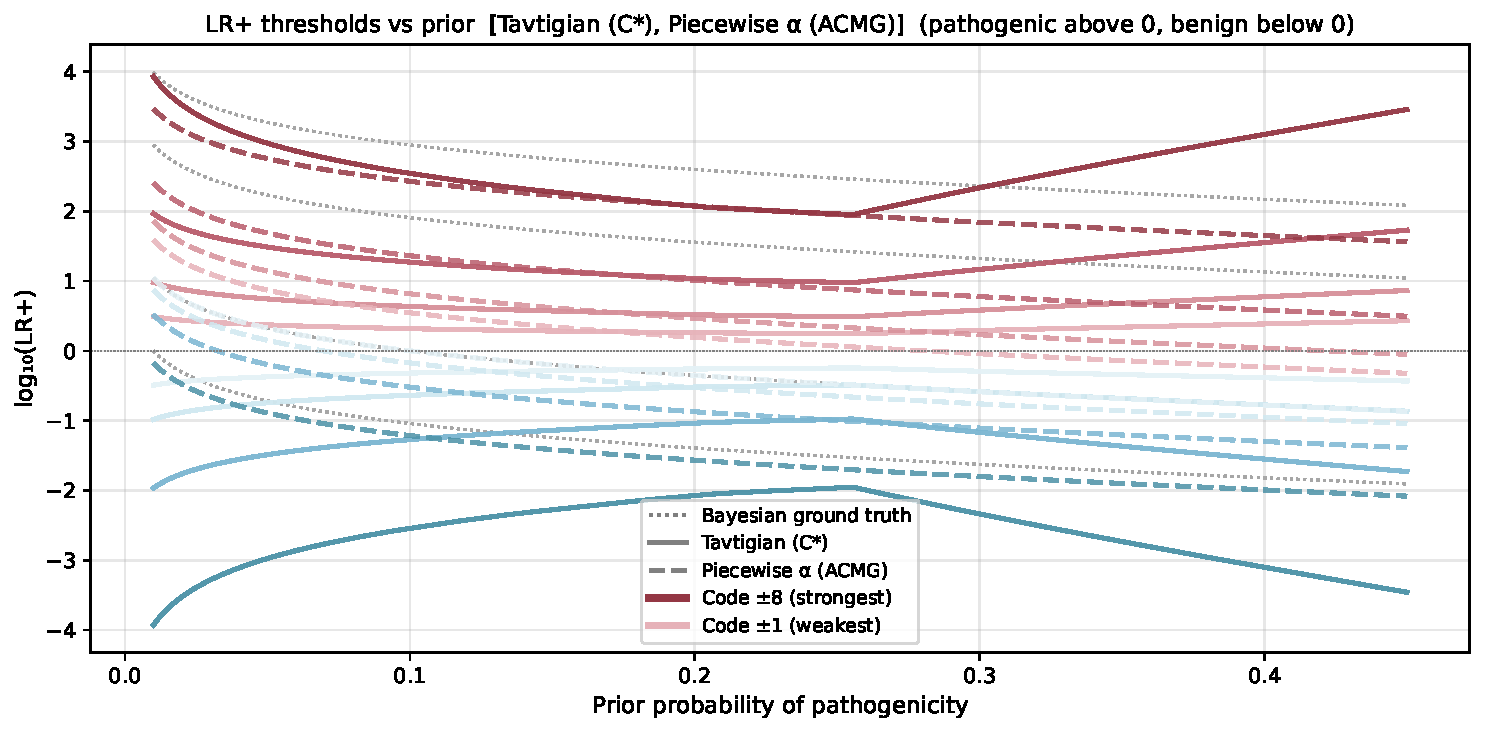
\includegraphics[width=0.92\textwidth]{figures/lr_thresholds.pdf}
  \caption{LR$^+$ thresholds for evidence codes 1, 2, 4, 8 (Su, M, S, VS)
           vs.\ gene-specific prior.
           Tavtigian (solid): follows $C^{*T/8}$; shows a non-monotone
           artefact near $p \approx 0.25$ where $C^*$ passes through its
           minimum, and a large spike at $p = 0.45$ where benign combination
           rules drive $C^*$ to 2876.
           Piecewise (dashed): varies smoothly; thresholds are prior-adaptive
           and produce exact posteriors at each evidence boundary.
           Dotted lines: analytical Bayesian thresholds (continuous ground truth).
           Warm colours = pathogenic codes; cool colours = benign codes.}
  \label{fig:lr_thresholds}
\end{figure}

\begin{figure}[p]
  \centering
  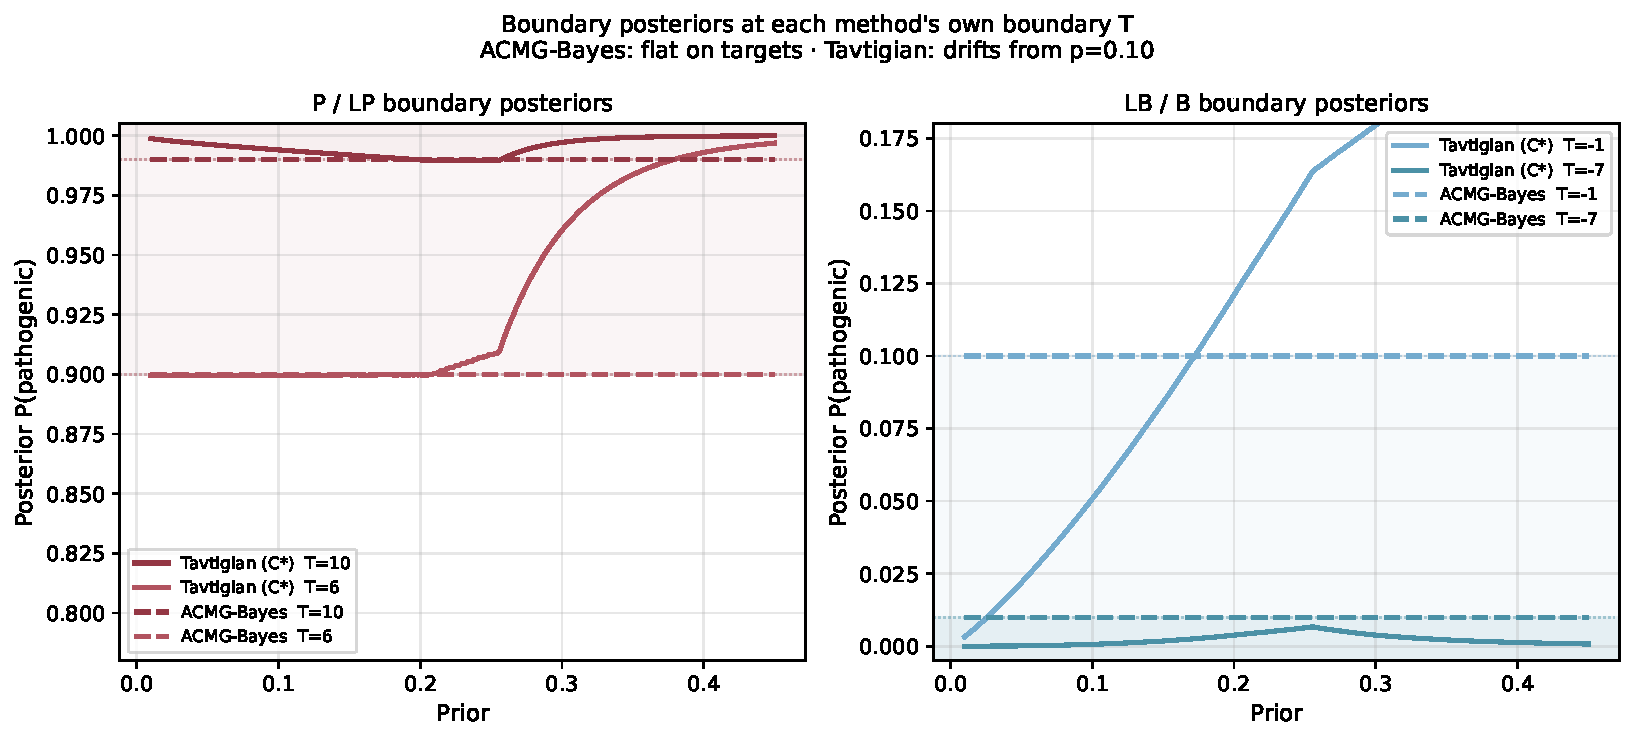
\includegraphics[width=0.92\textwidth]{figures/boundary_posteriors.pdf}
  \caption{Posterior probability at each method's classification boundary
           $T$ value vs.\ gene-specific prior.
           Piecewise (dashed): flat at all four targets by construction.
           Tavtigian (solid): well-calibrated for LP at priors $\leq 0.25$
           but severely miscalibrated for LB and B boundaries across the
           full prior range; anomalous over-calibration at $p \approx 0.45$.}
  \label{fig:boundary_posteriors}
\end{figure}

\begin{figure}[p]
  \centering
  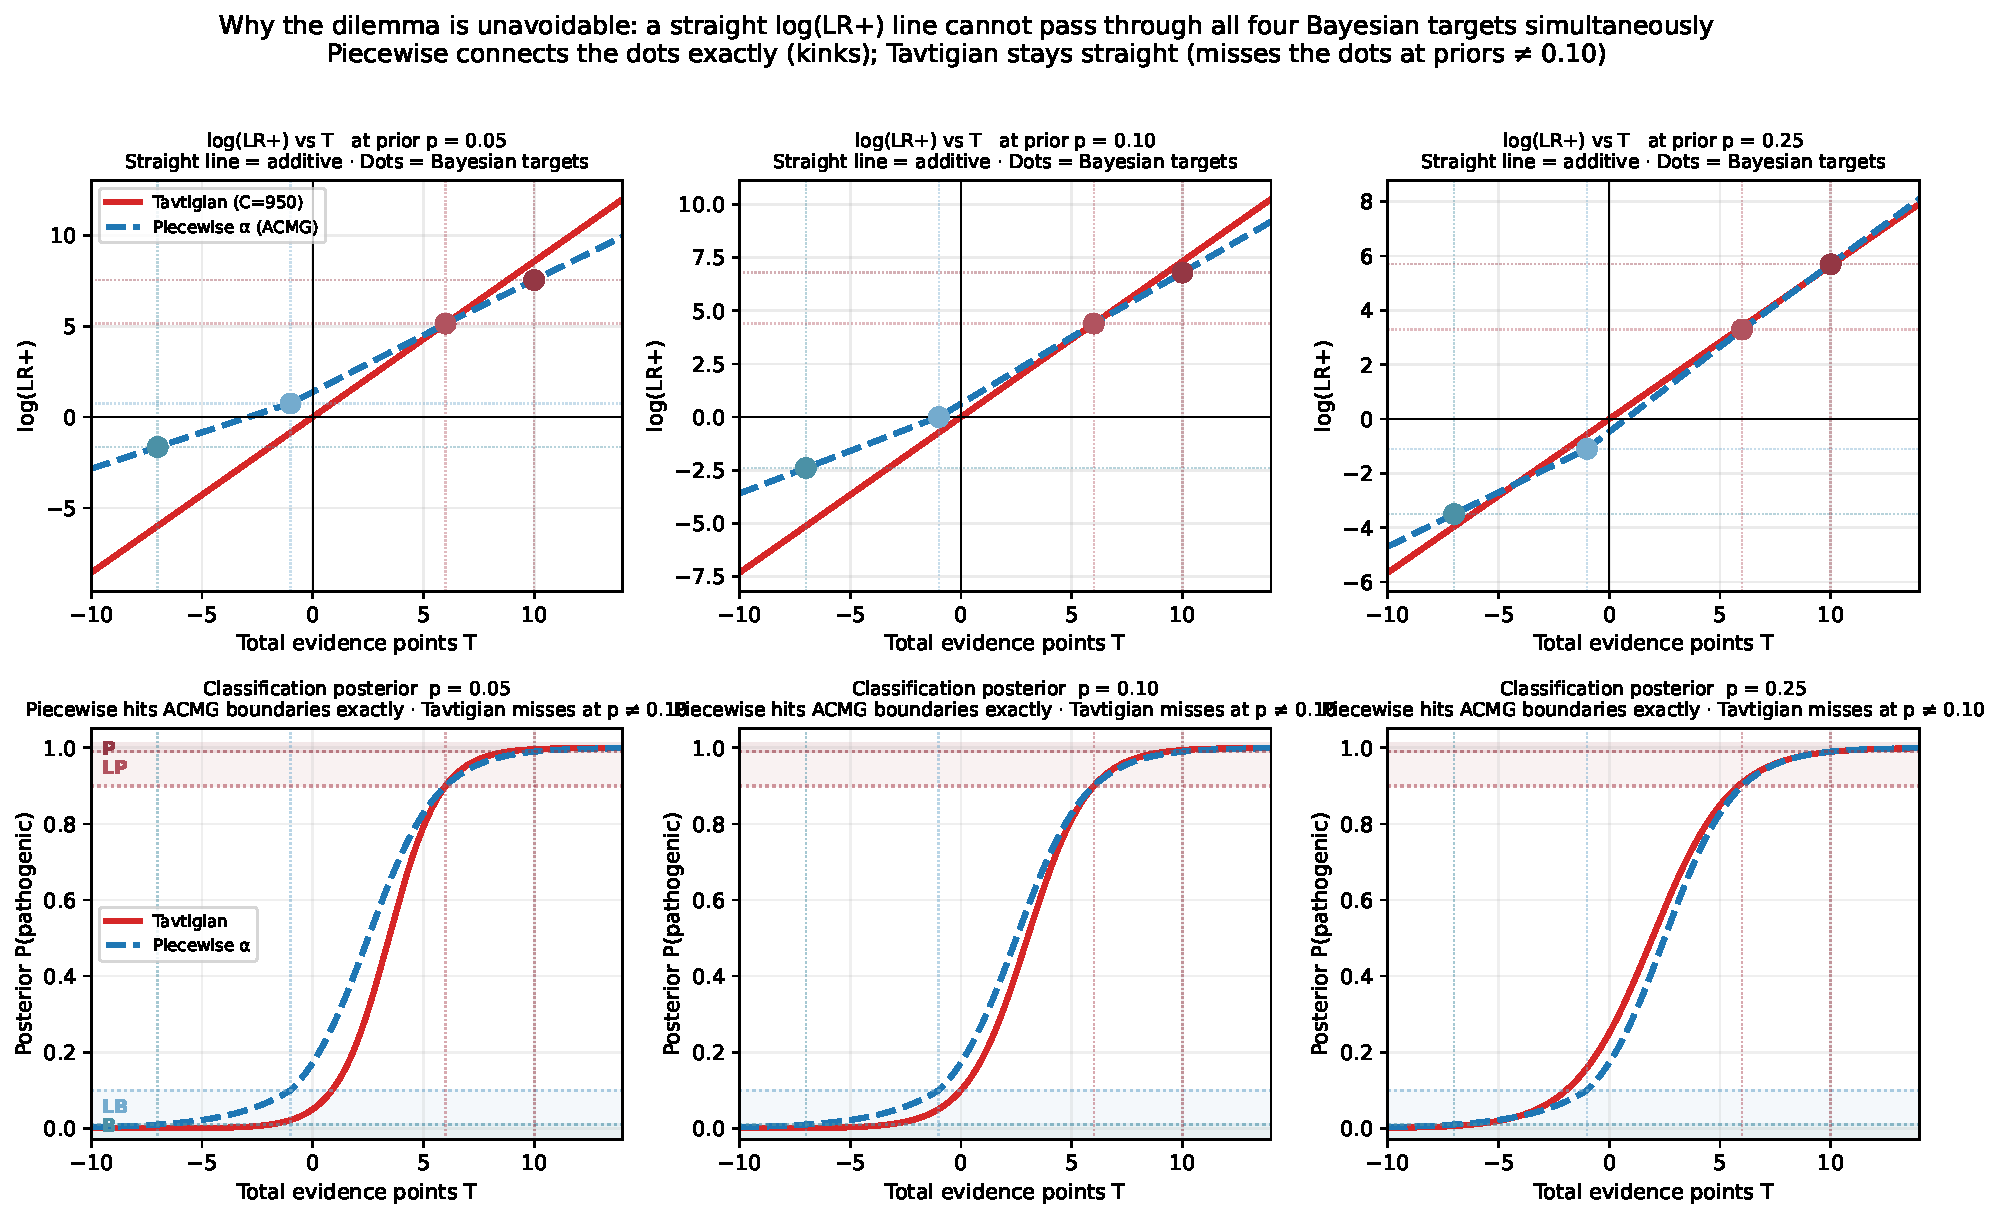
\includegraphics[width=0.95\textwidth]{figures/slope_geometry.pdf}
  \caption{$\log\lrp$ vs.\ total evidence points $T$ at three prior values.
           Coloured dots indicate the exact Bayesian target $\log\lrp$
           at each of the four classification boundaries.
           Tavtigian (red): a single straight line that passes through all
           four dots only at $p = 0.10$.
           Piecewise (blue): a kinked line that passes through all four dots
           at every prior by translating vertically.
           Lower panels: the corresponding posterior probability curves;
           piecewise reaches each ACMG boundary exactly, Tavtigian drifts.}
  \label{fig:slope_geometry}
\end{figure}

\begin{figure}[p]
  \centering
  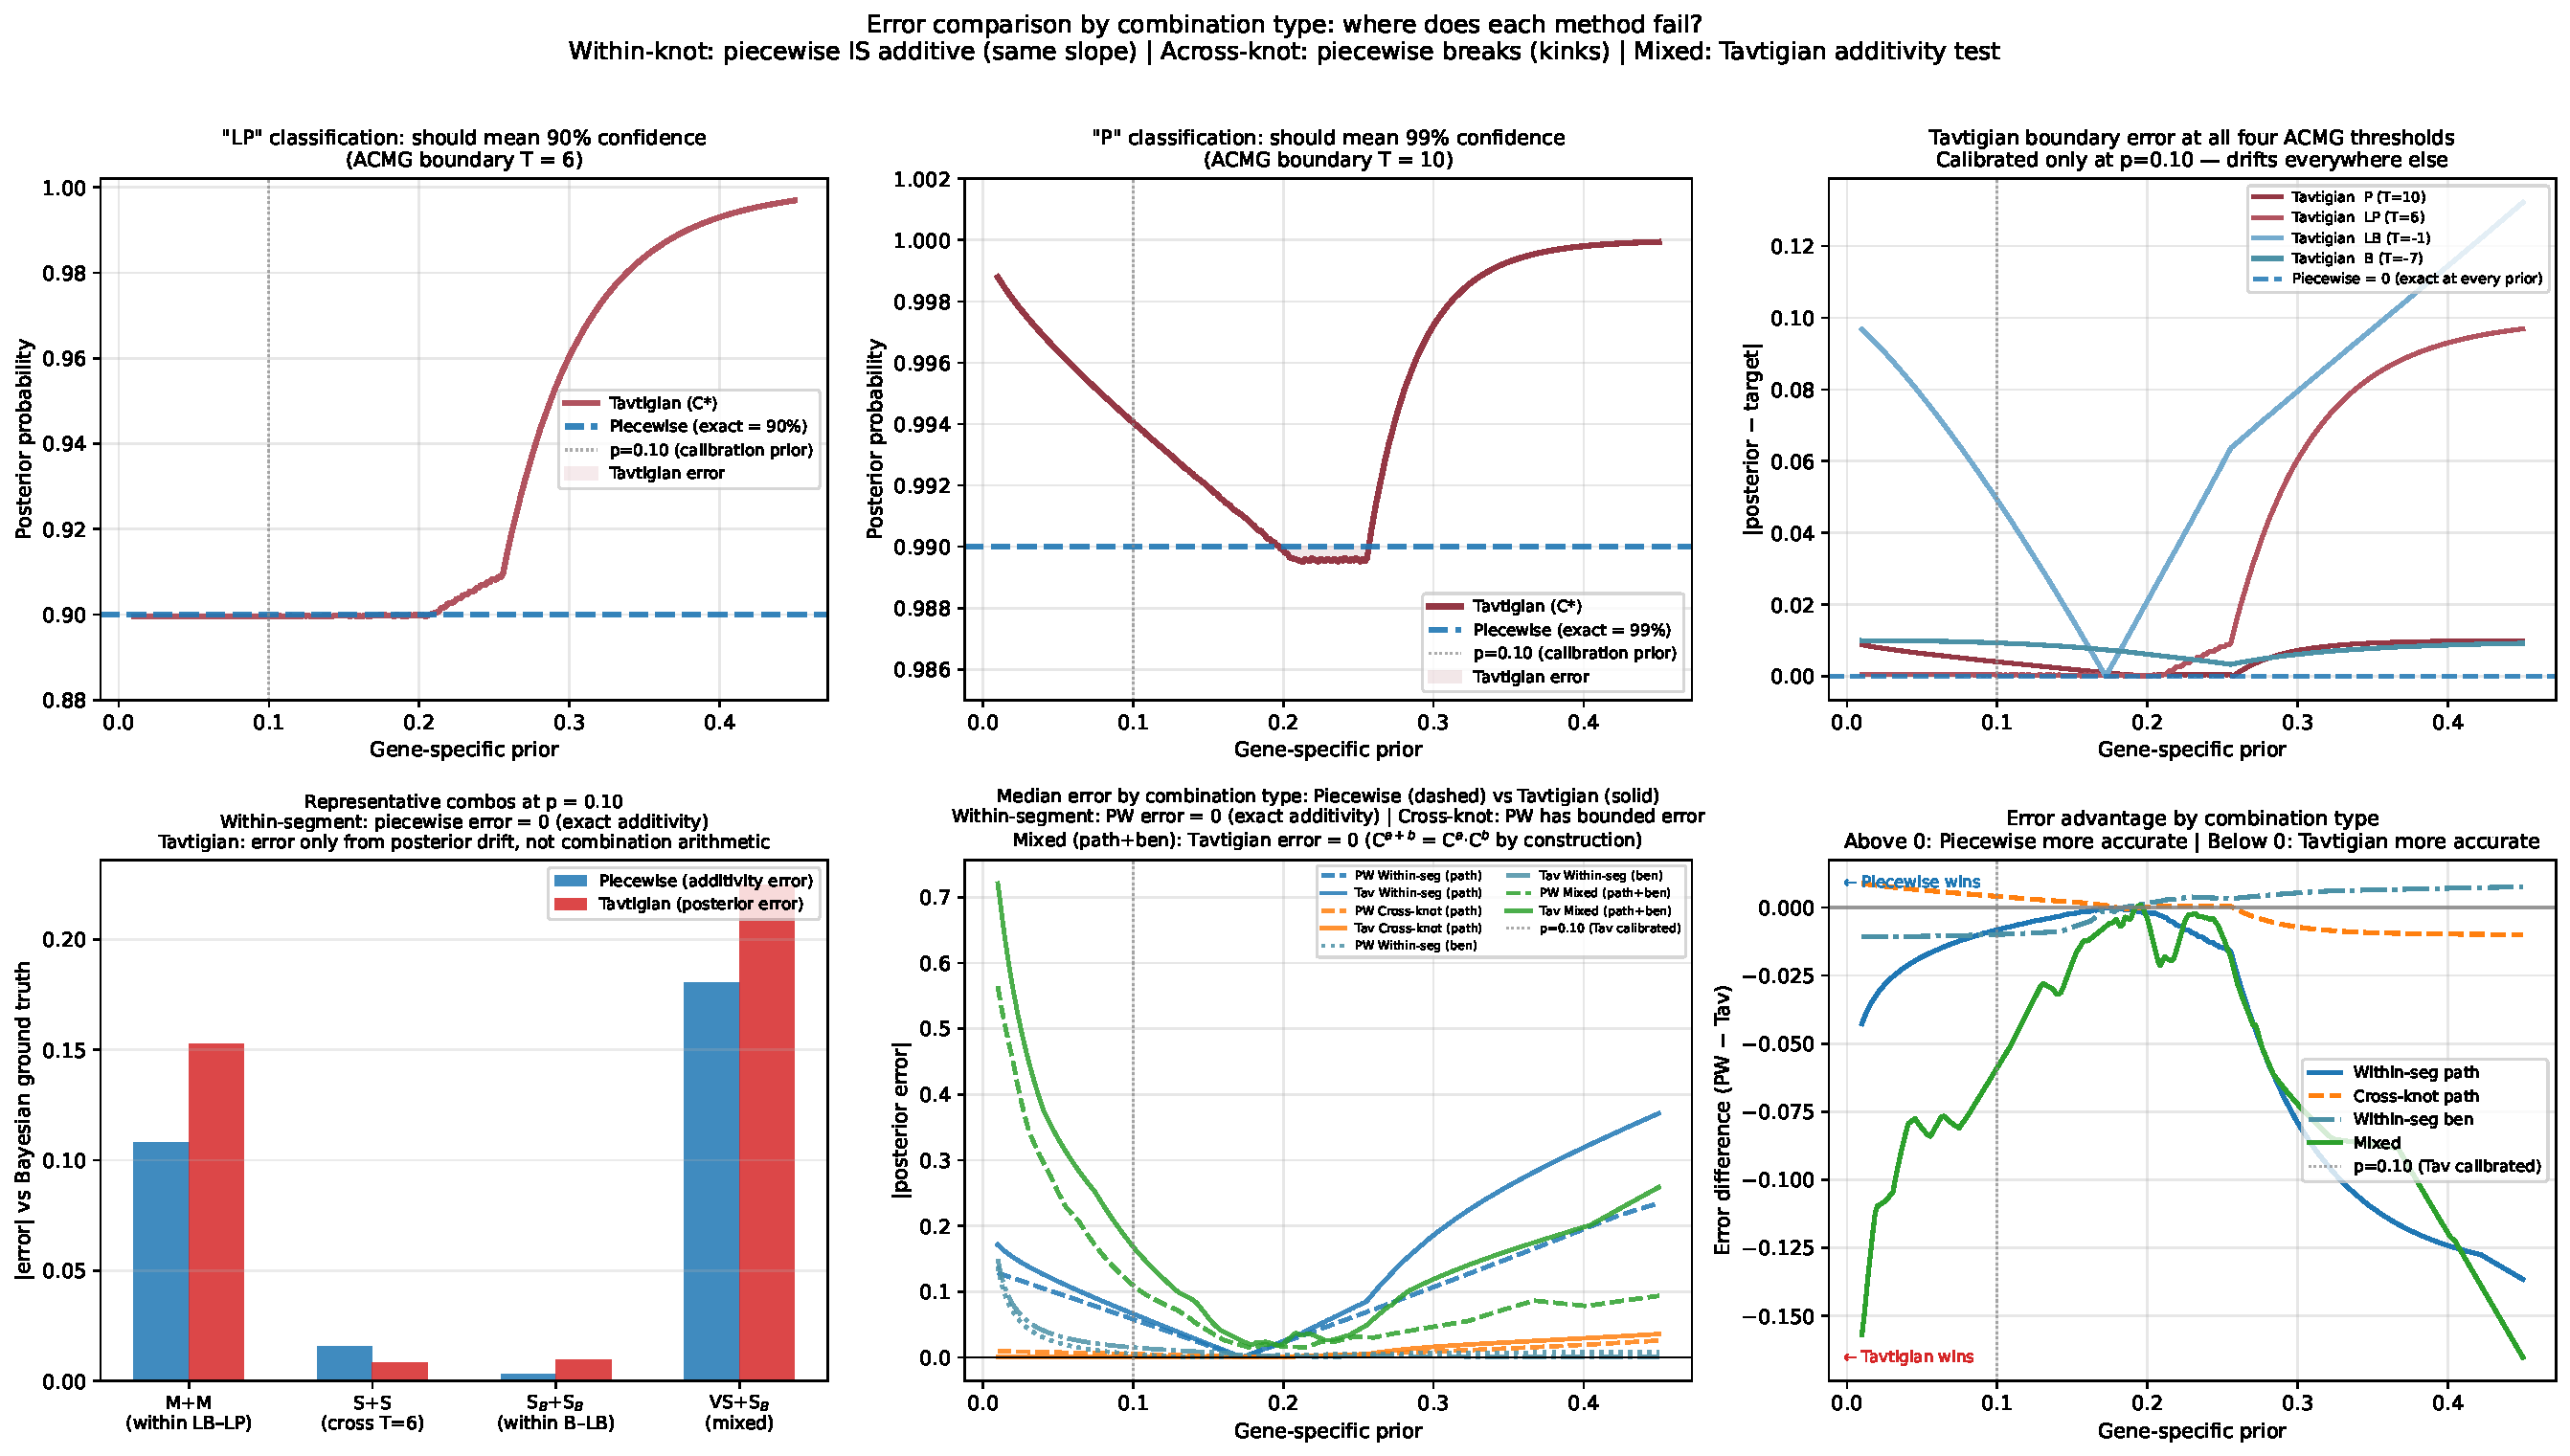
\includegraphics[width=0.98\textwidth]{figures/additivity_by_type.pdf}
  \caption{Evidence combination errors stratified by type.
           \emph{Top row}: single-assay boundary posteriors showing
           Tavtigian drift and piecewise exactness.
           \emph{Bottom left}: representative per-type errors at $p = 0.10$;
           both methods measured against the same Bayesian ground truth.
           \emph{Bottom middle}: median per-type combination errors
           vs.\ prior (piecewise dashed, Tavtigian solid).
           \emph{Bottom right}: error advantage (piecewise $-$ Tavtigian);
           positive = piecewise more accurate.}
  \label{fig:additivity_by_type}
\end{figure}

\begin{figure}[p]
  \centering
  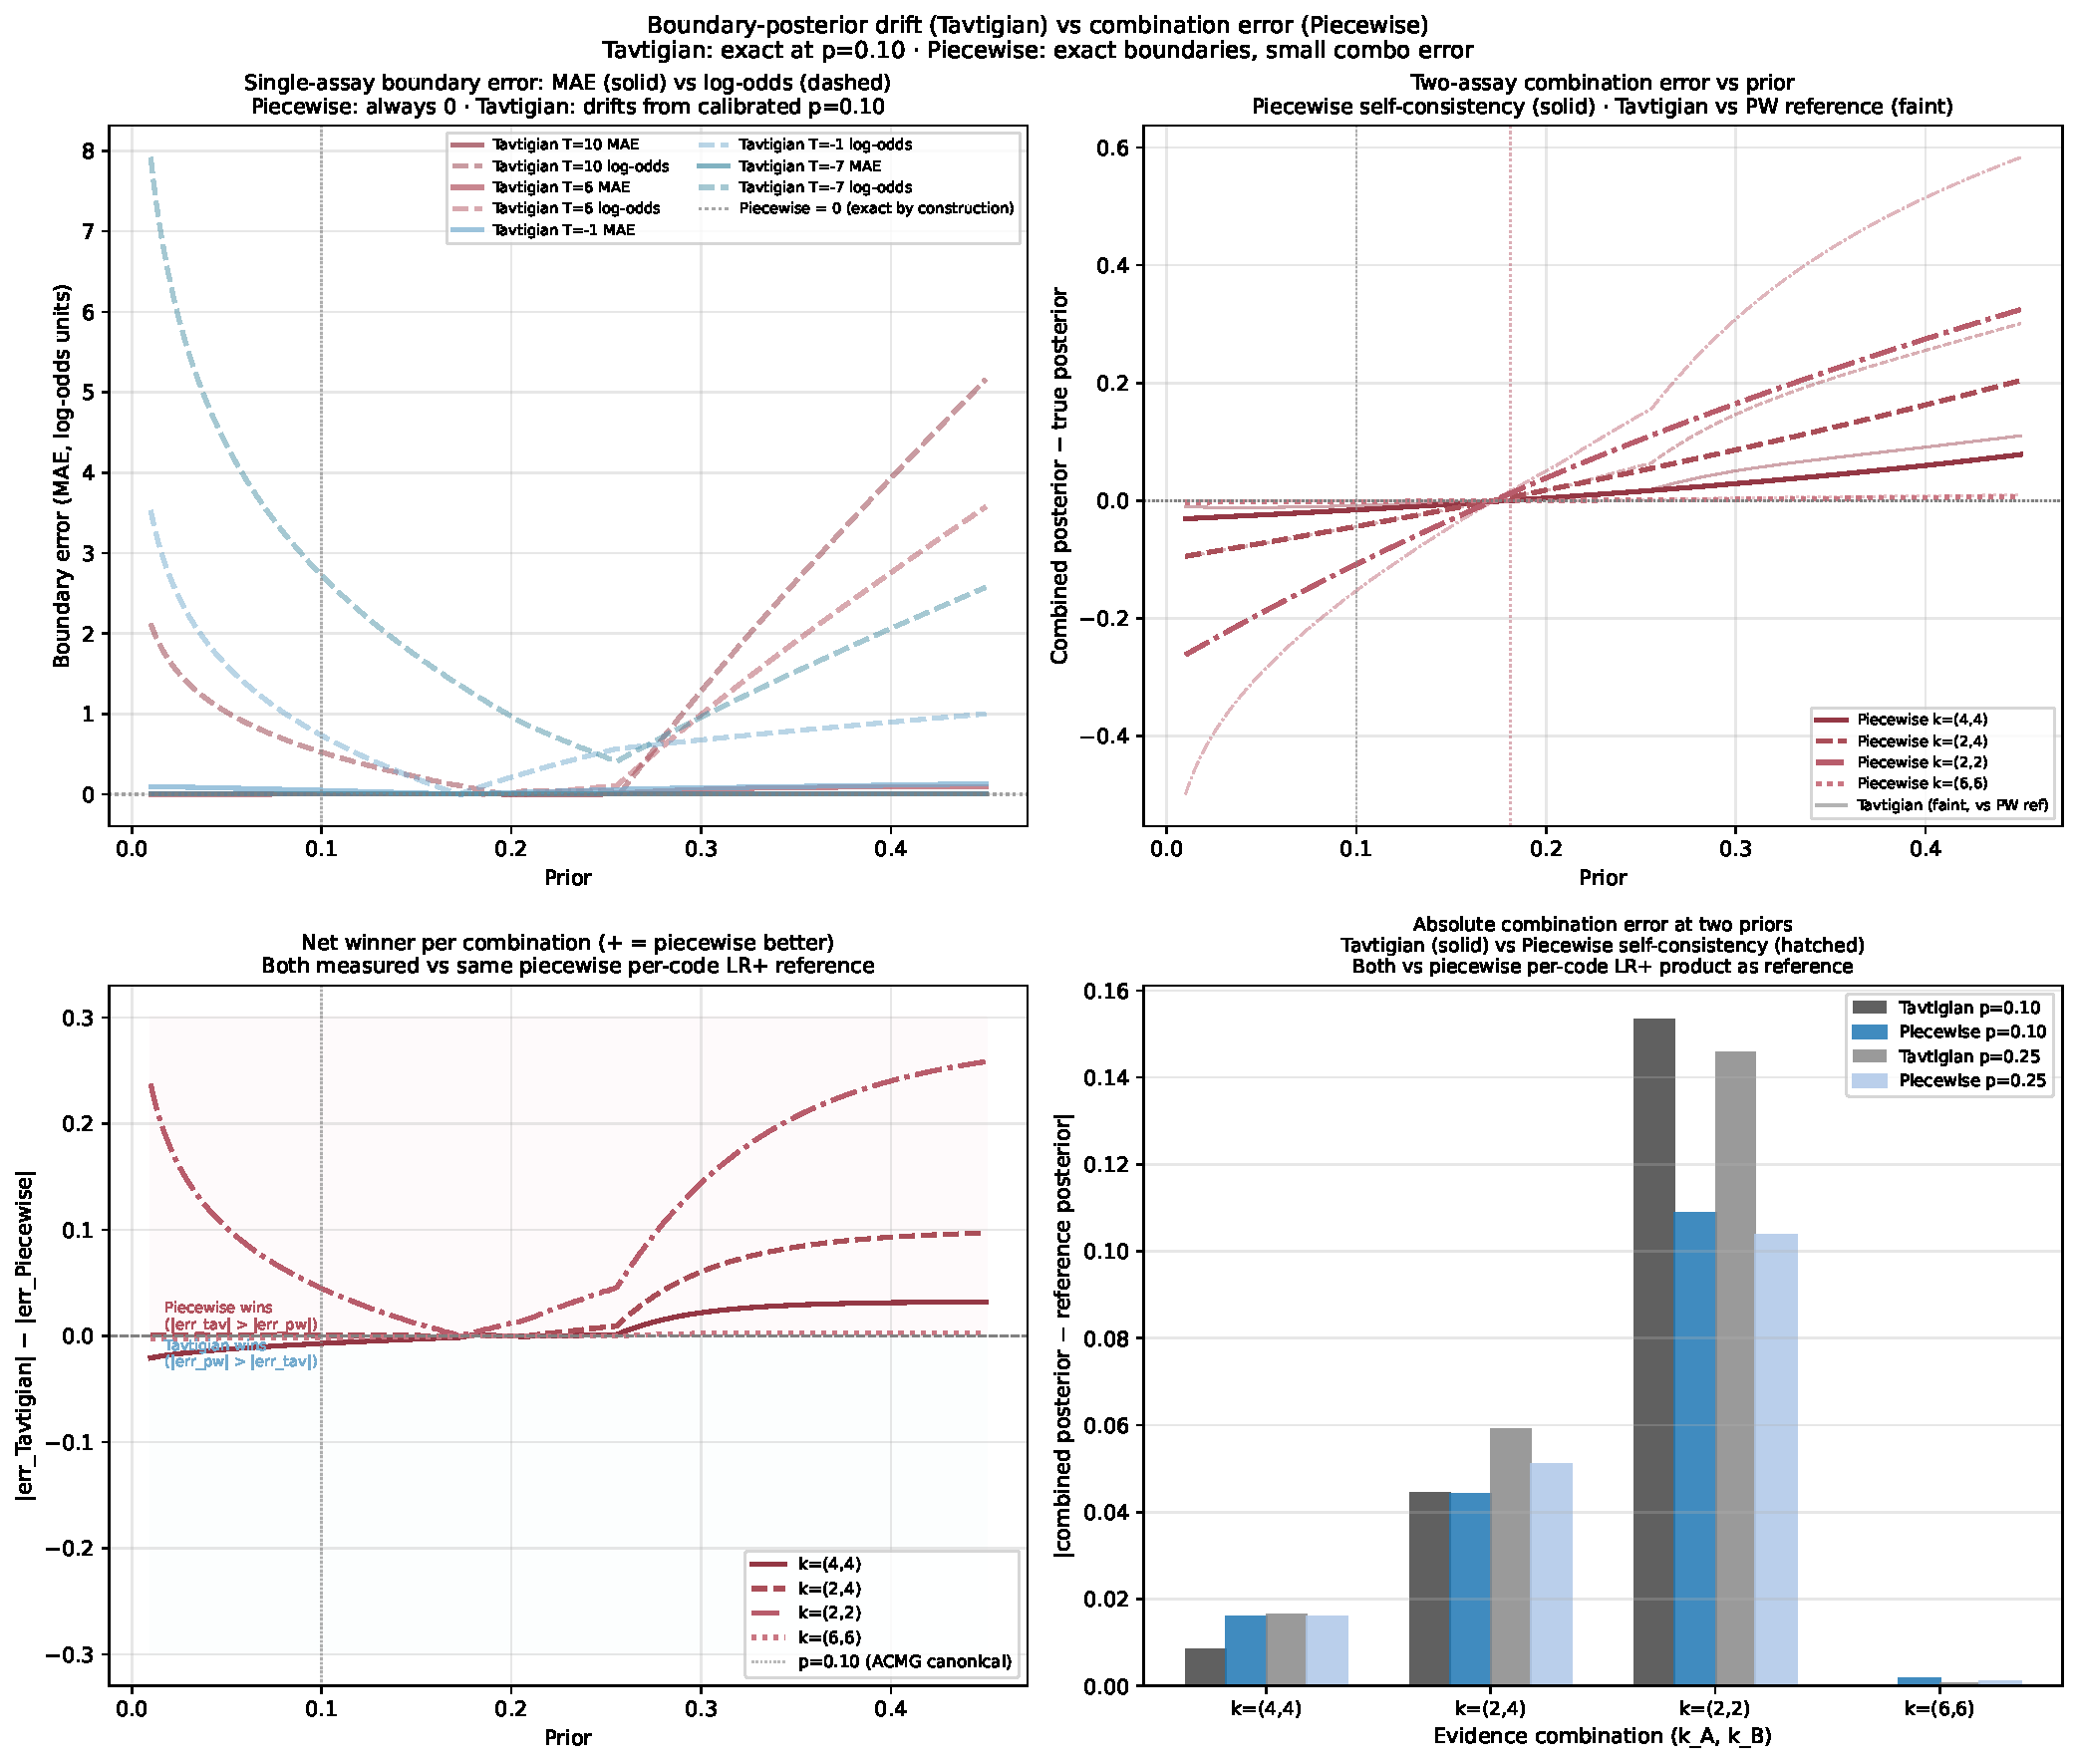
\includegraphics[width=0.95\textwidth]{figures/error_comparison.pdf}
  \caption{Single-assay boundary errors for both methods using two error
           metrics: MAE in posterior probability (solid) and absolute
           log-odds error $|\mathrm{logit}(\hat{p}) - \mathrm{logit}(\mathrm{target})|$
           (dashed).
           Piecewise = 0 at all boundaries by construction.
           The log-odds metric reveals the true severity of Tavtigian's
           benign-boundary miscalibration at low priors, which MAE
           substantially understates.}
  \label{fig:error_comparison}
\end{figure}

% ------------------------------------------------------------------
\clearpage
\appendix

\section*{Supplementary: evidence tier point system and combination rules}

\begin{table}[h]
\centering
\caption{ACMG/AMP combination rules in the modified Tavtigian point system
         \cite{tavtigian2018modeling, Tavtigian2020}.
         Points: Su\,=\,1, M\,=\,2, S\,=\,4, VS\,=\,8;
         Su$_B$\,=\,$-1$, S$_B$\,=\,$-4$ (standard ACMG benign tiers only).
         $^\dagger$Modified rule: original ACMG classifies VS+M as LP and
         2S as P; both are internally inconsistent at $p=0.10$, so following
         Tavtigian et al.\ they are swapped.
         All calculations use the modified (swapped) rules.}
\label{tab:rules}
\begin{tabular}{lll}
\toprule
Category & Combination & Points \\
\midrule
P  & VS $+$ S                                          & 12 \\
P  & VS $+$ 2M                                         & 12 \\
P  & VS $+$ M $+$ Su                                   & 11 \\
P  & VS $+$ M $^\dagger$                               & 10 \\
P  & S $+$ 3M                                          & 10 \\
P  & S $+$ 2M $+$ 2Su                                  & 10 \\
P  & S $+$ M $+$ 4Su                                   & 10 \\
\midrule
LP & S $+$ M                                           &  6 \\
LP & S $+$ 2Su                                         &  6 \\
LP & 3M                                                &  6 \\
LP & 2M $+$ 2Su                                        &  6 \\
LP & M $+$ 4Su                                         &  6 \\
LP & 2S $^\dagger$                                     &  8 \\
\midrule
LB & S$_B$ $+$ Su$_B$                                  & $-5$ \\
LB & 2Su$_B$                                           & $-2$ \\
B  & 2S$_B$                                            & $-8$ \\
\bottomrule
\end{tabular}
\end{table}

\section*{Supplementary: combination error tables}
\label{sec:supplement}

The following tables list the posterior combination errors for all
evidence pairs at priors $p \in \{0.01, 0.10, 0.25, 0.45\}$.
PW = piecewise additivity error; Tav = Tavtigian posterior error, both
measured against the Bayesian posterior from the piecewise per-code
LR$^+$ product.
Standard ACMG pathogenic tiers: Su$=1$, M$=2$, S$=4$, VS$=8$;
codes 3,5,6,7 are intermediate strengths not corresponding to named tiers.
Standard ACMG benign tiers: Su$_B=-1$, S$_B=-4$;
M$_B$ ($-2$, $^\dagger$) and VS$_B$ ($-8$, $^\dagger$) are non-standard
hypothetical extensions.

% This file is auto-generated by generate_figures.py

\begin{longtable}{llr @{\hspace{0.8em}} rr @{\hspace{0.8em}} rr @{\hspace{0.8em}} rr @{\hspace{0.8em}} rr}
\caption{Combination errors for all pathogenic code pairs. $k_A \leq k_B$, both in $\{1,2,3,4,5,6,7,8\}$. Codes 3,5,6,7 are intermediate strengths not corresponding to named ACMG tiers; codes 1,2,4,8 = Su, M, S, VS. PW = piecewise additivity error; Tav = Tavtigian posterior error. Both measured vs.\ the Bayesian posterior from the piecewise per-code LR$^+$ product.} \label{tab:s_path} \\
\toprule
$k_A$ & $k_B$ & $T$ & \multicolumn{2}{c}{$p=0.01$} & \multicolumn{2}{c}{$p=0.1$} & \multicolumn{2}{c}{$p=0.25$} & \multicolumn{2}{c}{$p=0.45$} \\
 & & & \textbf{PW} & \textbf{Tav} & \textbf{PW} & \textbf{Tav} & \textbf{PW} & \textbf{Tav} & \textbf{PW} & \textbf{Tav} \\
\midrule \endfirsthead
\toprule
$k_A$ & $k_B$ & $T$ & \multicolumn{2}{c}{$p=0.01$} & \multicolumn{2}{c}{$p=0.1$} & \multicolumn{2}{c}{$p=0.25$} & \multicolumn{2}{c}{$p=0.45$} \\
 & & & \textbf{PW} & \textbf{Tav} & \textbf{PW} & \textbf{Tav} & \textbf{PW} & \textbf{Tav} & \textbf{PW} & \textbf{Tav} \\
\midrule \endhead
\midrule \multicolumn{11}{r}{\small continued\ldots} \\ \endfoot
\bottomrule \endlastfoot
Su & Su & 2 & \textbf{3.03} & 5.04 & \textbf{0.628} & 1.05 & \textbf{0.471} & 0.817 & \textbf{1.37} & 3.47 \\
Su & M & 3 & \textbf{3.03} & 4.54 & \textbf{0.628} & 0.942 & \textbf{0.471} & 0.754 & \textbf{1.37} & 3.84 \\
Su & Su+M? & 4 & \textbf{3.03} & 4.04 & \textbf{0.628} & 0.838 & \textbf{0.471} & 0.691 & \textbf{1.37} & 4.21 \\
Su & S & 5 & \textbf{3.03} & 3.53 & \textbf{0.628} & 0.733 & \textbf{0.471} & 0.629 & \textbf{1.37} & 4.58 \\
Su & Su+S? & 6 & \textbf{3.03} & 3.03 & \textbf{0.628} & 0.629 & \textbf{0.471} & 0.566 & \textbf{1.37} & 4.94 \\
Su & M+S? & 7 & 3.05 & \textbf{2.53} & 0.656 & \textbf{0.524} & \textbf{0.443} & 0.504 & \textbf{1.34} & 5.31 \\
Su & Su+M+S? & 8 & 3.05 & \textbf{2.00} & 0.656 & \textbf{0.392} & \textbf{0.443} & 0.470 & \textbf{1.34} & 5.71 \\
Su & VS & 9 & 3.05 & \textbf{1.46} & 0.656 & \textbf{0.259} & 0.443 & \textbf{0.435} & \textbf{1.34} & 6.10 \\
M & M & 4 & \textbf{3.03} & 4.04 & \textbf{0.628} & 0.838 & \textbf{0.471} & 0.691 & \textbf{1.37} & 4.21 \\
M & Su+M? & 5 & \textbf{3.03} & 3.53 & \textbf{0.628} & 0.733 & \textbf{0.471} & 0.629 & \textbf{1.37} & 4.58 \\
M & S & 6 & \textbf{3.03} & 3.03 & \textbf{0.628} & 0.629 & \textbf{0.471} & 0.566 & \textbf{1.37} & 4.94 \\
M & Su+S? & 7 & 3.05 & \textbf{2.53} & 0.656 & \textbf{0.524} & \textbf{0.443} & 0.504 & \textbf{1.34} & 5.31 \\
M & M+S? & 8 & 3.08 & \textbf{2.02} & 0.684 & \textbf{0.420} & \textbf{0.414} & 0.441 & \textbf{1.31} & 5.68 \\
M & Su+M+S? & 9 & 3.08 & \textbf{1.49} & 0.684 & \textbf{0.287} & 0.414 & \textbf{0.407} & \textbf{1.31} & 6.08 \\
M & VS & 10 & 3.08 & \textbf{0.961} & 0.684 & \textbf{0.154} & 0.414 & \textbf{0.373} & \textbf{1.31} & 6.47 \\
Su+M? & Su+M? & 6 & \textbf{3.03} & 3.03 & \textbf{0.628} & 0.629 & \textbf{0.471} & 0.566 & \textbf{1.37} & 4.94 \\
Su+M? & S & 7 & 3.05 & \textbf{2.53} & 0.656 & \textbf{0.524} & \textbf{0.443} & 0.504 & \textbf{1.34} & 5.31 \\
Su+M? & Su+S? & 8 & 3.08 & \textbf{2.02} & 0.684 & \textbf{0.420} & \textbf{0.414} & 0.441 & \textbf{1.31} & 5.68 \\
Su+M? & M+S? & 9 & 3.11 & \textbf{1.52} & 0.713 & \textbf{0.315} & 0.386 & \textbf{0.379} & \textbf{1.28} & 6.05 \\
Su+M? & Su+M+S? & 10 & 3.11 & \textbf{0.989} & 0.713 & \textbf{0.183} & 0.386 & \textbf{0.344} & \textbf{1.28} & 6.44 \\
Su+M? & VS & 11 & 3.11 & \textbf{0.458} & 0.713 & \textbf{0.050} & 0.386 & \textbf{0.310} & \textbf{1.28} & 6.84 \\
S & S & 8 & 3.08 & \textbf{2.02} & 0.684 & \textbf{0.420} & \textbf{0.414} & 0.441 & \textbf{1.31} & 5.68 \\
S & Su+S? & 9 & 3.11 & \textbf{1.52} & 0.713 & \textbf{0.315} & 0.386 & \textbf{0.379} & \textbf{1.28} & 6.05 \\
S & M+S? & 10 & 3.14 & \textbf{1.02} & 0.741 & \textbf{0.211} & 0.358 & \textbf{0.316} & \textbf{1.26} & 6.41 \\
S & Su+M+S? & 11 & 3.14 & \textbf{0.486} & 0.741 & \textbf{0.078} & 0.358 & \textbf{0.282} & \textbf{1.26} & 6.81 \\
S & VS & 12 & 3.14 & \textbf{0.046} & 0.741 & \textbf{0.055} & 0.358 & \textbf{0.248} & \textbf{1.26} & 7.21 \\
Su+S? & Su+S? & 10 & 3.14 & \textbf{1.02} & 0.741 & \textbf{0.211} & 0.358 & \textbf{0.316} & \textbf{1.26} & 6.41 \\
Su+S? & M+S? & 11 & 3.17 & \textbf{0.514} & 0.769 & \textbf{0.106} & 0.329 & \textbf{0.254} & \textbf{1.23} & 6.78 \\
Su+S? & Su+M+S? & 12 & 3.17 & \textbf{0.017} & 0.769 & \textbf{0.026} & 0.329 & \textbf{0.219} & \textbf{1.23} & 7.18 \\
Su+S? & VS & 13 & 3.17 & \textbf{0.549} & 0.769 & \textbf{0.159} & 0.329 & \textbf{0.185} & \textbf{1.23} & 7.57 \\
M+S? & M+S? & 12 & 3.20 & \textbf{0.011} & 0.798 & \textbf{0.002} & 0.301 & \textbf{0.191} & \textbf{1.20} & 7.15 \\
M+S? & Su+M+S? & 13 & 3.20 & \textbf{0.521} & 0.798 & \textbf{0.131} & 0.301 & \textbf{0.157} & \textbf{1.20} & 7.55 \\
M+S? & VS & 14 & 3.20 & \textbf{1.05} & 0.798 & \textbf{0.264} & 0.301 & \textbf{0.123} & \textbf{1.20} & 7.94 \\
Su+M+S? & Su+M+S? & 14 & 3.20 & \textbf{1.05} & 0.798 & \textbf{0.264} & 0.301 & \textbf{0.123} & \textbf{1.20} & 7.94 \\
Su+M+S? & VS & 15 & 3.20 & \textbf{1.58} & 0.798 & \textbf{0.396} & 0.301 & \textbf{0.088} & \textbf{1.20} & 8.34 \\
VS & VS & 16 & 3.20 & \textbf{2.12} & 0.798 & \textbf{0.529} & 0.301 & \textbf{0.054} & \textbf{1.20} & 8.73 \\
\end{longtable}

\begin{longtable}{llr @{\hspace{0.8em}} rr @{\hspace{0.8em}} rr @{\hspace{0.8em}} rr @{\hspace{0.8em}} rr}
\caption{Combination errors for benign code pairs. Standard ACMG benign tiers are Su$_B$ ($-1$ pt) and S$_B$ ($-4$ pt); M$_B$ ($-2$ pt, $\dagger$) and VS$_B$ ($-8$ pt, $\dagger$) are non-standard hypothetical extensions included for completeness. Negative $T$ totals indicate net benign evidence.} \label{tab:s_ben} \\
\toprule
$k_A$ & $k_B$ & $T$ & \multicolumn{2}{c}{$p=0.01$} & \multicolumn{2}{c}{$p=0.1$} & \multicolumn{2}{c}{$p=0.25$} & \multicolumn{2}{c}{$p=0.45$} \\
 & & & \textbf{PW} & \textbf{Tav} & \textbf{PW} & \textbf{Tav} & \textbf{PW} & \textbf{Tav} & \textbf{PW} & \textbf{Tav} \\
\midrule \endfirsthead
\toprule
$k_A$ & $k_B$ & $T$ & \multicolumn{2}{c}{$p=0.01$} & \multicolumn{2}{c}{$p=0.1$} & \multicolumn{2}{c}{$p=0.25$} & \multicolumn{2}{c}{$p=0.45$} \\
 & & & \textbf{PW} & \textbf{Tav} & \textbf{PW} & \textbf{Tav} & \textbf{PW} & \textbf{Tav} & \textbf{PW} & \textbf{Tav} \\
\midrule \endhead
\midrule \multicolumn{11}{r}{\small continued\ldots} \\ \endfoot
\bottomrule \endlastfoot
Su$_B$ & Su$_B$ & -2 & \textbf{2.80} & 7.06 & \textbf{0.400} & 1.46 & \textbf{0.699} & 1.07 & \textbf{1.60} & 2.00 \\
Su$_B$ & M$_B$† & -3 & \textbf{2.80} & 7.79 & \textbf{0.400} & 1.80 & \textbf{0.699} & 0.901 & 1.60 & \textbf{1.41} \\
Su$_B$ & S$_B$ & -5 & \textbf{2.80} & 9.25 & \textbf{0.400} & 2.46 & 0.699 & \textbf{0.570} & 1.60 & \textbf{0.214} \\
Su$_B$ & VS$_B$† & -9 & \textbf{2.80} & 12.18 & \textbf{0.400} & 3.79 & 0.699 & \textbf{0.092} & \textbf{1.60} & 2.17 \\
M$_B$† & M$_B$† & -4 & \textbf{2.80} & 8.52 & \textbf{0.400} & 2.13 & \textbf{0.699} & 0.736 & 1.60 & \textbf{0.810} \\
M$_B$† & S$_B$ & -6 & \textbf{2.80} & 9.98 & \textbf{0.400} & 2.79 & 0.699 & \textbf{0.404} & 1.60 & \textbf{0.381} \\
M$_B$† & VS$_B$† & -10 & \textbf{2.80} & 12.91 & \textbf{0.400} & 4.13 & 0.699 & \textbf{0.258} & \textbf{1.60} & 2.76 \\
S$_B$ & S$_B$ & -8 & \textbf{2.80} & 11.45 & \textbf{0.400} & 3.46 & 0.699 & \textbf{0.073} & 1.60 & \textbf{1.57} \\
S$_B$ & VS$_B$† & -12 & \textbf{2.80} & 14.37 & \textbf{0.400} & 4.79 & 0.699 & \textbf{0.589} & \textbf{1.60} & 3.96 \\
VS$_B$† & VS$_B$† & -16 & \textbf{2.80} & 15.33 & \textbf{0.400} & 6.12 & \textbf{0.699} & 1.25 & \textbf{1.60} & 6.34 \\
\end{longtable}

\begin{longtable}{llr @{\hspace{0.8em}} rr @{\hspace{0.8em}} rr @{\hspace{0.8em}} rr @{\hspace{0.8em}} rr}
\caption{Combination errors for mixed (pathogenic $+$ benign) code pairs. $k_A > 0$ (pathogenic tier), $k_B < 0$ (benign tier). Tavtigian has zero internal combination error for mixed evidence by construction ($C^{a+b} = C^a \cdot C^b$), but its per-code LR$^+$ thresholds are miscalibrated at non-canonical priors, so the posterior errors are still large.} \label{tab:s_mixed} \\
\toprule
$k_A$ & $k_B$ & $T$ & \multicolumn{2}{c}{$p=0.01$} & \multicolumn{2}{c}{$p=0.1$} & \multicolumn{2}{c}{$p=0.25$} & \multicolumn{2}{c}{$p=0.45$} \\
 & & & \textbf{PW} & \textbf{Tav} & \textbf{PW} & \textbf{Tav} & \textbf{PW} & \textbf{Tav} & \textbf{PW} & \textbf{Tav} \\
\midrule \endfirsthead
\toprule
$k_A$ & $k_B$ & $T$ & \multicolumn{2}{c}{$p=0.01$} & \multicolumn{2}{c}{$p=0.1$} & \multicolumn{2}{c}{$p=0.25$} & \multicolumn{2}{c}{$p=0.45$} \\
 & & & \textbf{PW} & \textbf{Tav} & \textbf{PW} & \textbf{Tav} & \textbf{PW} & \textbf{Tav} & \textbf{PW} & \textbf{Tav} \\
\midrule \endhead
\midrule \multicolumn{11}{r}{\small continued\ldots} \\ \endfoot
\bottomrule \endlastfoot
Su & Su$_B$ & 0 & \textbf{3.03} & 6.05 & \textbf{0.628} & 1.26 & \textbf{0.471} & 0.942 & \textbf{1.37} & 2.74 \\
Su & M$_B$† & -1 & \textbf{3.25} & 6.78 & \textbf{0.856} & 1.59 & \textbf{0.243} & 0.776 & \textbf{1.14} & 2.14 \\
Su & S$_B$ & -3 & \textbf{3.25} & 8.25 & \textbf{0.856} & 2.25 & \textbf{0.243} & 0.445 & 1.14 & \textbf{0.950} \\
Su & VS$_B$† & -7 & \textbf{3.25} & 11.17 & \textbf{0.856} & 3.58 & 0.243 & \textbf{0.217} & \textbf{1.14} & 1.43 \\
M & Su$_B$ & 1 & \textbf{3.03} & 5.55 & \textbf{0.628} & 1.15 & \textbf{0.471} & 0.879 & \textbf{1.37} & 3.11 \\
M & M$_B$† & 0 & \textbf{3.25} & 6.28 & \textbf{0.856} & 1.48 & \textbf{0.243} & 0.714 & \textbf{1.14} & 2.51 \\
M & S$_B$ & -2 & \textbf{3.48} & 7.74 & \textbf{1.08} & 2.15 & \textbf{0.015} & 0.382 & \textbf{0.913} & 1.32 \\
M & VS$_B$† & -6 & \textbf{3.48} & 10.67 & \textbf{1.08} & 3.48 & \textbf{0.015} & 0.280 & \textbf{0.913} & 1.07 \\
S & Su$_B$ & 3 & \textbf{3.03} & 4.54 & \textbf{0.628} & 0.942 & \textbf{0.471} & 0.754 & \textbf{1.37} & 3.84 \\
S & M$_B$† & 2 & \textbf{3.25} & 5.27 & \textbf{0.856} & 1.27 & \textbf{0.243} & 0.588 & \textbf{1.14} & 3.24 \\
S & S$_B$ & 0 & \textbf{3.71} & 6.74 & \textbf{1.31} & 1.94 & \textbf{0.214} & 0.257 & \textbf{0.684} & 2.05 \\
S & VS$_B$† & -4 & \textbf{3.94} & 9.66 & \textbf{1.54} & 3.27 & 0.442 & \textbf{0.405} & 0.456 & \textbf{0.330} \\
VS & Su$_B$ & 7 & 3.00 & \textbf{2.47} & 0.599 & \textbf{0.468} & \textbf{0.499} & 0.560 & \textbf{1.40} & 5.37 \\
VS & M$_B$† & 6 & \textbf{3.20} & 3.20 & \textbf{0.799} & 0.800 & \textbf{0.299} & 0.395 & \textbf{1.20} & 4.77 \\
VS & S$_B$ & 4 & \textbf{3.65} & 4.67 & \textbf{1.26} & 1.47 & 0.157 & \textbf{0.064} & \textbf{0.741} & 3.58 \\
VS & VS$_B$† & 0 & \textbf{4.57} & 7.59 & \textbf{2.17} & 2.80 & 1.07 & \textbf{0.599} & \textbf{0.172} & 1.20 \\
\end{longtable}


% ------------------------------------------------------------------
\bibliographystyle{unsrtnat}
\begin{thebibliography}{9}

\bibitem{richards2015standards}
Richards, S., et al.
\newblock Standards and guidelines for the interpretation of sequence variants.
\newblock \textit{Genet Med}, 17(5):405--424, 2015.

\bibitem{tavtigian2018modeling}
Tavtigian, S.~V., et al.
\newblock Modeling the ACMG/AMP variant classification guidelines as a
  Bayesian classification framework.
\newblock \textit{Genet Med}, 20(9):1054--1060, 2018.

\bibitem{Tavtigian2020}
Tavtigian, S.~V., et al.
\newblock Fitting a naturally scaled point system to the ACMG/AMP variant
  classification guidelines.
\newblock \textit{Hum Mutat}, 41(10):1734--1737, 2020.

\bibitem{brnich2020recommendations}
Brnich, S.~E., et al.
\newblock Recommendations for application of the functional evidence PS3/BS3
  criterion using the ACMG/AMP sequence variant interpretation framework.
\newblock \textit{Genome Med}, 12(1):3, 2019.

\bibitem{pejaver2022calibration}
Pejaver, V., et al.
\newblock Calibration of computational tools for missense variant pathogenicity
  classification and ClinGen recommendations for PP3/BP4 criteria.
\newblock \textit{Am J Hum Genet}, 109(12):2163--2177, 2022.

\bibitem{Harrison2019}
Harrison, S.~M.\ and Rehm, H.~L.
\newblock Is `likely pathogenic' really 90\% likely? Reclassification data in
  ClinVar.
\newblock \textit{Genome Med}, 11(1):72, 2019.

\bibitem{igvf_pp}
Tejura, M., et al.
\newblock A scalable approach to resolving variants of uncertain significance.
\newblock \textit{bioRxiv} 2026.02.14.705848, 2026.

\bibitem{Glas2003}
Glas, A.~S., et al.
\newblock The diagnostic odds ratio: a single indicator of test performance.
\newblock \textit{J Clin Epidemiol}, 56(11):1129--1135, 2003.

\end{thebibliography}

\end{document}
